% =====================================================================
%  Team 58 -- Type 1: Research Project
%  An AI-Driven, Blockchain-Anchored Cyber Deception Framework
%  Beamer source. Compile with:  tectonic PPT.tex     (or pdflatex x2)
% =====================================================================
\documentclass[aspectratio=169,11pt]{beamer}

% ---------- packages -------------------------------------------------
\usepackage[T1]{fontenc}
\usepackage[utf8]{inputenc}
\usepackage{lmodern}
\usepackage{booktabs}
\usepackage{array}
\usepackage{colortbl}
\usepackage{tikz}
\usepackage{pgfplots}
\usepackage{amssymb}
\usepackage{ragged2e}
\usepackage{adjustbox}
\newcolumntype{L}[1]{>{\raggedright\arraybackslash}p{#1}}
\newcolumntype{R}[1]{>{\raggedleft\arraybackslash}p{#1}}
\pgfplotsset{compat=1.17}
\usetikzlibrary{positioning,arrows.meta,fit,backgrounds,calc,shapes.geometric,shadows.blur}

% ---------- theme skeleton ------------------------------------------
\usetheme{default}
\usecolortheme{default}
\setbeamertemplate{navigation symbols}{}
\setbeamertemplate{itemize items}[circle]
\setbeamertemplate{enumerate items}[default]
\setbeamertemplate{section in toc}[sections numbered]

% ---------- palette --------------------------------------------------
\definecolor{navy}{HTML}{12304F}
\definecolor{steel}{HTML}{2C5F8A}
\definecolor{teal}{HTML}{0E7C7B}
\definecolor{amber}{HTML}{B8860B}
\definecolor{crimson}{HTML}{A32B2B}
\definecolor{ink}{HTML}{1B1B1F}
\definecolor{mist}{HTML}{EEF2F6}
\definecolor{mist2}{HTML}{DCE5EE}
\definecolor{grayline}{HTML}{9AA6B2}

\setbeamercolor{normal text}{fg=ink}
\setbeamercolor{structure}{fg=navy}
\setbeamercolor{frametitle}{fg=white,bg=navy}
\setbeamercolor{title}{fg=navy}
\setbeamercolor{itemize item}{fg=teal}
\setbeamercolor{itemize subitem}{fg=steel}
\setbeamercolor{block title}{fg=white,bg=teal}
\setbeamercolor{block body}{fg=ink,bg=mist}
\setbeamercolor{block title alerted}{fg=white,bg=crimson}
\setbeamercolor{block body alerted}{fg=ink,bg=mist}
\setbeamerfont{frametitle}{size=\large,series=\bfseries}
\setbeamerfont{block title}{size=\small,series=\bfseries}

% ---------- MARGINS --------------------------------------------------
% Generous, symmetric side margins; frametitle band with breathing room.
\setbeamersize{text margin left=0.85cm, text margin right=0.85cm}

\makeatletter
\setbeamertemplate{frametitle}{%
  \nointerlineskip%
  \begin{beamercolorbox}[wd=\paperwidth,sep=0pt]{frametitle}%
    \vskip0.24cm%
    \hbox{\hspace{0.85cm}%
    \begin{minipage}{\dimexpr\paperwidth-1.7cm\relax}
      \raggedright\usebeamerfont{frametitle}\insertframetitle%
      \ifx\insertframesubtitle\@empty\else
        \\[2.5pt]{\normalfont\scriptsize\insertframesubtitle}%
      \fi
    \end{minipage}%
    \hspace{0.85cm}}%
    \vskip0.24cm%
  \end{beamercolorbox}%
  \vspace{0.26cm}%
}
\makeatother

% ---------- footline -------------------------------------------------
\setbeamertemplate{footline}{%
  \hbox{%
  \begin{beamercolorbox}[wd=.62\paperwidth,ht=2.4ex,dp=1.1ex,leftskip=0.85cm]{}%
    \color{grayline}\scriptsize Team 58 \; | \; AI-Driven, Blockchain-Anchored Cyber Deception
  \end{beamercolorbox}%
  \begin{beamercolorbox}[wd=.38\paperwidth,ht=2.4ex,dp=1.1ex,rightskip=0.85cm]{}%
    \hfill\color{grayline}\scriptsize\insertshortsubtitle\;\;\textbf{\insertframenumber}/\inserttotalframenumber
  \end{beamercolorbox}}%
  \vskip2pt%
}

% ---------- helper macros -------------------------------------------
\newcommand{\srcnote}[1]{\par\vspace{3pt}{\raggedleft\scriptsize\color{grayline}\itshape #1\par}}
\newcommand{\hl}[1]{\textcolor{navy}{\textbf{#1}}}
\newcommand{\bad}[1]{\textcolor{crimson}{\textbf{#1}}}
\newcommand{\good}[1]{\textcolor{teal}{\textbf{#1}}}
\newcommand{\tick}{{\color{teal}$\checkmark$}}
\newcommand{\cross}{{\color{crimson}$\times$}}
\newcommand{\takeaway}[1]{%
  \vspace{3pt}%
  \begin{beamercolorbox}[wd=\dimexpr\textwidth-10pt\relax,sep=5pt,rounded=true]{block body}%
    {\color{navy}\bfseries\scriptsize TAKEAWAY\;\;}{\scriptsize #1}%
  \end{beamercolorbox}}

% table row colours
\newcommand{\hdrow}{\rowcolor{navy}}
\newcommand{\hc}[1]{\textcolor{white}{\textbf{#1}}}
\newcommand{\altrow}{\rowcolor{mist}}
\newcommand{\ourrow}{\rowcolor{mist2}}

% tikz styles
\tikzset{
  box/.style   ={rectangle, rounded corners=2pt, draw=navy, line width=0.6pt,
                 fill=white, align=center, font=\scriptsize, inner sep=3.5pt},
  edgebox/.style={box, fill=navy!12, draw=navy},
  decoy/.style ={box, fill=steel!12, draw=steel},
  ai/.style    ={box, fill=teal!14, draw=teal},
  chain/.style ={box, fill=amber!18, draw=amber!80!black},
  attacker/.style={box, fill=crimson!12, draw=crimson, font=\scriptsize\bfseries},
  flow/.style  ={-{Stealth[length=4pt]}, draw=navy!75, line width=0.7pt},
  flowb/.style ={-{Stealth[length=4pt]}, draw=teal!85, line width=0.7pt, dashed},
  lbl/.style   ={font=\tiny\itshape, color=navy!75, inner sep=1.5pt, fill=white},
  zone/.style  ={rounded corners=4pt, draw=grayline, dashed, line width=0.6pt,
                 inner sep=7pt},
  ztitle/.style={font=\tiny\bfseries, color=grayline},
}

% =====================================================================
\title{An AI-Driven, Blockchain-Anchored Cyber Deception Framework for Adaptive Honeypot Defense}
\subtitle{Type 1: Research Project}
\author{Team 58}
\institute{Guide: Dr.\ Radhika G}
\date{}

\begin{document}

% ============================== TITLE ================================
{\setbeamertemplate{footline}{}
\begin{frame}[plain]
  \vspace{0.15cm}
  \begin{center}
    {\scriptsize\color{teal}\bfseries TYPE 1: RESEARCH PROJECT \quad$\cdot$\quad TEAM NUMBER 58}\\[6pt]
    {\color{navy}\rule{0.86\textwidth}{1.1pt}}\\[7pt]
    {\Large\color{navy}\bfseries An AI-Driven, Blockchain-Anchored}\\[3pt]
    {\Large\color{navy}\bfseries Cyber Deception Framework}\\[4pt]
    {\normalsize\color{steel} for Adaptive Honeypot Defense}\\[5pt]
    {\color{navy}\rule{0.86\textwidth}{1.1pt}}
  \end{center}
  \vspace{0.10cm}
  \begin{center}
  {\scriptsize
  \begin{tabular}{@{}clll@{}}
    \toprule
    \textbf{S.No} & \textbf{Register Number} & \textbf{Student Name} \\
    \midrule
    1 & CB.SC.U4CSE23111 & B Guru Sai Prasad \\
    2 & CB.SC.U4CSE23127 & N Surya Tejaswar \\
    3 & CB.SC.U4CSE23129 & N Sisir Reddy \\
    4 & CB.SC.U4CSE23611 & C Pranav Sharma \\
    5 & CB.SC.U4CSE23644 & R Vishnu Sathwick \\
    \bottomrule
  \end{tabular}}
  \end{center}
  \vspace{0.15cm}
  \begin{center}{\small\color{navy}\bfseries Guide: Dr.\ Radhika G}\end{center}
\end{frame}}

% ============================== ROADMAP ==============================
\begin{frame}{Roadmap of the Presentation}
  \vspace{-2pt}
  \begin{columns}[T,onlytextwidth]
    \begin{column}{0.485\textwidth}
      \footnotesize
      \textbf{\color{navy}Part A --- The Problem \& The Design}\\[2pt]
      \begin{enumerate}\setlength\itemsep{0.8pt}
        \item Problem statement and motivation
        \item Objectives and research gaps
        \item Comparison against existing honeypots
        \item System architecture (one picture)
        \item Life of a single attacker request
        \item The five decoy services
        \item The three-tier AI response engine
        \item Blockchain-anchored logging
        \item Implementation stack
      \end{enumerate}
    \end{column}
    \begin{column}{0.485\textwidth}
      \footnotesize
      \textbf{\color{navy}Part B --- What We Measured}\\[2pt]
      \begin{enumerate}\setlength\itemsep{0.8pt}\setcounter{enumi}{9}
        \item Evaluation methodology
        \item Module 1: deception engine (4 runs)
        \item Module 2: tamper-evident audit trail
        \item Module 3: AI verdict accountability
        \item Module 4: federated threat intelligence
        \item Honest failures we found
        \item Project status --- 70\% complete
        \item Discussion, limitations, future work
      \end{enumerate}
    \end{column}
  \end{columns}
  \takeaway{We built \emph{one} deception platform, then evaluated it as \emph{four} separate research modules. Part B is the evidence that the design in Part A actually works --- and where it does not.}
\end{frame}

% ============================== PROBLEM ==============================
\begin{frame}{Problem Statement}
  \footnotesize
  Traditional honeypots rely on \hl{static, deterministic response tables} --- efficient at scale,
  but fragile against fingerprinting.
  \vspace{3pt}
  \begin{itemize}\setlength\itemsep{3pt}
    \item \textbf{Fingerprintable by design.} Prior work shows automated probing can distinguish
      static honeypots (Cowrie, Kippo, Dionaea) from real systems with near-perfect accuracy
      in a \emph{single} packet exchange.
    \item \textbf{Single-protocol LLM deception.} Existing LLM-backed honeypots (shelLM,
      HoneyGPT) are concentrated on SSH/terminal sessions only --- no shared framework
      spans multiple heterogeneous protocols.
    \item \textbf{Untrustworthy forensic logs.} A compromised honeypot host can have its own
      logs silently edited by the attacker, destroying the evidentiary value of captured telemetry.
    \item \textbf{No accountability for AI decisions.} As LLMs move into the triage loop, a wrong
      verdict can be quietly edited afterwards --- an error laundered into something authoritative.
  \end{itemize}
  \takeaway{A honeypot must be \emph{believable}, \emph{broad}, and its evidence must be \emph{provable} --- current systems deliver at most one of the three.}
\end{frame}

% ============================== OBJECTIVE ============================
\begin{frame}{Objectives}
  \footnotesize
  To build a deployable, multi-protocol deception framework that stays convincing under
  sustained probing and produces a \hl{tamper-evident audit trail}.
  \vspace{3pt}
  \begin{itemize}\setlength\itemsep{2pt}
    \item \textbf{Cover five distinct attack surfaces} --- SSH, an internal AI API, PostgreSQL,
      an Ethereum JSON-RPC node, and Jenkins CI/CD --- behind \emph{one} shared response engine.
    \item \textbf{Stay fast where it can, smart where it must.} Answer routine traffic
      ($\approx$80\%) at millisecond latency via a static path; reserve LLM generation for
      genuinely novel input.
    \item \textbf{Make every interaction context-aware.} Replace canned responses with an
      LLM engine that is session-history-aware and intent-classified.
    \item \textbf{Anchor forensic integrity independently of the host.} Hash and commit every
      log entry to a separate blockchain, so tampering is detectable even if the honeypot
      itself is compromised.
    \item \textbf{Hold the AI itself accountable.} Anchor the classifier's \emph{verdicts} too,
      and measure how often they are wrong.
    \item \textbf{Evaluate honestly.} Latency, throughput, diversity and realism as
      \emph{separate} axes across successively larger datasets --- reporting failures, not just
      favourable numbers.
  \end{itemize}
\end{frame}

% ============================== GAPS =================================
\begin{frame}{Research Gaps We Address}
  \footnotesize
  \begin{itemize}\setlength\itemsep{4pt}
    \item \textbf{LLM deception is single-protocol.} shelLM, HoneyGPT and related 2023--2025
      work apply LLM response generation only to SSH/terminal sessions; no prior system applies
      \emph{one} LLM engine uniformly across five heterogeneous protocol types.
    \item \textbf{Tamper-evident logging is generic, not honeypot-specific.} Blockchain
      hash-anchoring is established in digital forensics (evidence tracking, cloud VM
      investigation), but we found no honeypot-specific paper combining hash-anchoring
      with decoy logging.
    \item \textbf{Realism is rarely benchmarked rigorously.} Prior LLM-honeypot papers report a
      single self-evaluated accuracy figure (e.g.\ HoneyGPT's self-reported $\approx$96\%);
      few report latency/throughput trade-offs or scale-dependent failure modes.
    \item \textbf{AI triage output is treated as ground truth.} Work that adds an LLM classifier
      to security telemetry rarely asks what happens when the model is wrong --- or makes
      the wrong verdict independently verifiable after the fact.
    \item \textbf{Cross-honeypot correlation assumes a central hub.} MISP / STIX-TAXII designs
      make the aggregator the single machine an adversary must reach to blind the network.
  \end{itemize}
\end{frame}

% ============================== COMPARISON ===========================
\begin{frame}{Comparison Against Cited Systems}
  \par\vspace{2pt}
  \centering\scriptsize
  \setlength{\tabcolsep}{4pt}\renewcommand{\arraystretch}{1.02}
  \begin{tabular}{@{}L{1.65cm} L{1.85cm} L{3.6cm} L{2.95cm} L{2.15cm}@{}}
    \hdrow \hc{System} & \hc{Interaction} & \hc{AI / LLM Responses} & \hc{Protocols} & \hc{Tamper-evident}\\
    \altrow Cowrie & Medium/High & No (experimental single-tier LLM fallback) & SSH, Telnet & No\\
    T-Pot & Mixed (orchestrator) & No --- aggregation only & Broad (bundled daemons) & No\\
    \altrow Dionaea & Low--Medium & No & SMB, MySQL, SIP, FTP, TFTP & No\\
    shelLM & High (SSH only) & Yes --- full LLM shell session & SSH only & Not addressed\\
    \altrow HoneyGPT & High (terminal) & Yes --- GPT-3.5/4 via Cowrie proxy & SSH / terminal only & Not addressed\\
    \ourrow \textbf{This work} & \textbf{High, all 5} & \textbf{Yes --- 3-tier, session-aware, uniform across 5 protocols} & \textbf{SSH, AI API, SQL, Web3 RPC, CI/CD} & \textbf{Yes --- SHA-256 + Ethereum anchor}\\
    \bottomrule
  \end{tabular}
  \srcnote{Table I, paper Section II.F}
  \takeaway{We are the only row that is simultaneously multi-protocol, LLM-driven \emph{and} forensically verifiable.}
\end{frame}

% ============================== ARCHITECTURE =========================
\begin{frame}{System Architecture}
  \vspace{-5pt}
  \centering
  \begin{adjustbox}{max width=\textwidth, max totalheight=6.60cm, center}
  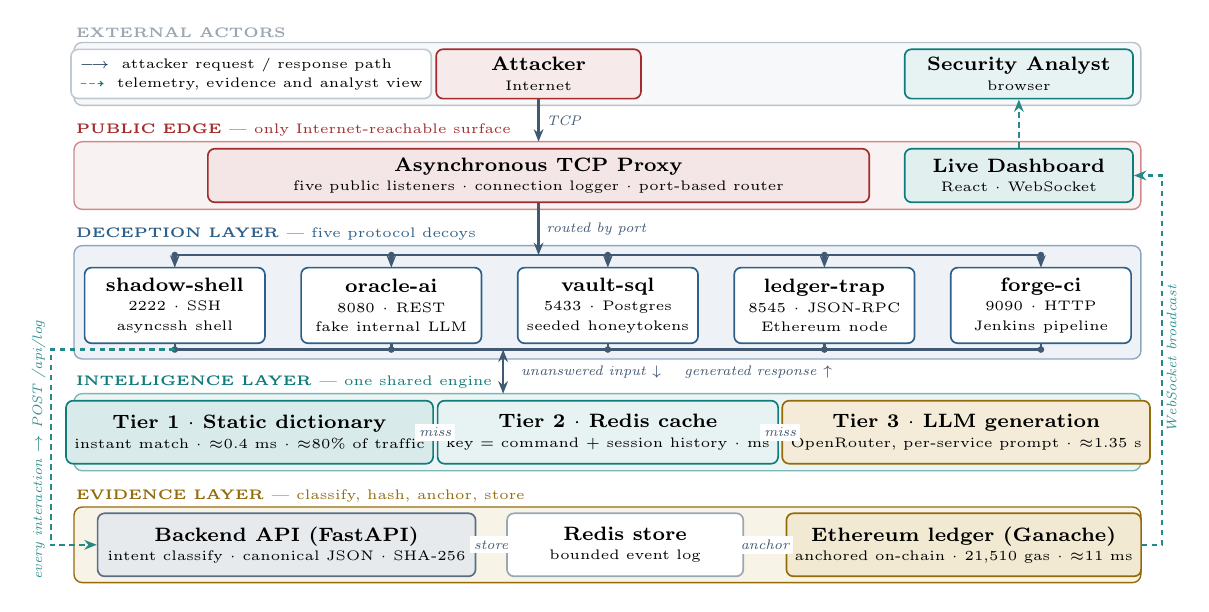
\begin{tikzpicture}[
      x=1cm, y=1cm, font=\scriptsize,
      band/.style     ={rounded corners=3pt, line width=0.5pt},
      bandlbl/.style  ={font=\tiny\bfseries, inner sep=0pt, anchor=south west},
      card/.style     ={rectangle, rounded corners=2.5pt, line width=0.6pt,
                        fill=white, align=center, inner sep=2pt, text width=2.15cm},
      wide/.style     ={rectangle, rounded corners=2.5pt, line width=0.6pt,
                        fill=white, align=center, inner sep=3pt},
      req/.style      ={-{Stealth[length=4.5pt,width=3.5pt]}, draw=navy!80, line width=0.85pt},
      rail/.style     ={draw=navy!80, line width=0.9pt},
      tel/.style      ={-{Stealth[length=4.5pt,width=3.5pt]}, draw=teal!90,
                        line width=0.85pt, dashed, dash pattern=on 2pt off 1.6pt},
      elbl/.style     ={font=\tiny\itshape, color=navy!80, inner sep=1.5pt, fill=white},
      tlbl/.style     ={font=\tiny\itshape, color=teal!85, inner sep=1.5pt, fill=white},
      dot/.style      ={circle, fill=navy!80, inner sep=0pt, minimum size=2.4pt},
    ]

    % =========================== BANDS ===================================
    \fill[band, fill=mist!55,     draw=grayline!70]     (0.60, 0.40) rectangle (14.15,-0.40);
    \fill[band, fill=crimson!6,   draw=crimson!55]      (0.60,-0.86) rectangle (14.15,-1.72);
    \fill[band, fill=steel!8,     draw=steel!55]        (0.60,-2.18) rectangle (14.15,-3.62);
    \fill[band, fill=teal!8,      draw=teal!55]         (0.60,-4.06) rectangle (14.15,-5.04);
    \fill[band, fill=amber!10,    draw=amber!80!black]  (0.60,-5.50) rectangle (14.15,-6.46);

    \node[bandlbl, color=grayline]      at (0.62, 0.46) {EXTERNAL ACTORS};
    \node[bandlbl, color=crimson]       at (0.62,-0.80) {PUBLIC EDGE \textnormal{--- only Internet-reachable surface}};
    \node[bandlbl, color=steel]         at (0.62,-2.12) {DECEPTION LAYER \textnormal{--- five protocol decoys}};
    \node[bandlbl, color=teal]          at (0.62,-4.00) {INTELLIGENCE LAYER \textnormal{--- one shared engine}};
    \node[bandlbl, color=amber!80!black]at (0.62,-5.44) {EVIDENCE LAYER \textnormal{--- classify, hash, anchor, store}};

    % =========================== BAND 1 : actors =========================
    \node[wide, draw=grayline!60, minimum width=4.4cm, minimum height=0.62cm, align=left, font=\tiny] (leg) at (2.85,0)
      {\textcolor{navy}{\bfseries$\longrightarrow$}\; attacker request / response path\\[1pt]
       \textcolor{teal}{\bfseries$\dashrightarrow$}\; telemetry, evidence and analyst view};
    \node[wide, draw=crimson, fill=crimson!10, minimum width=2.6cm, minimum height=0.62cm] (atk) at (6.50,0)
      {\textbf{Attacker}\\[-1pt]{\tiny Internet}};
    \node[wide, draw=teal, fill=teal!10, minimum width=2.9cm, minimum height=0.62cm] (analyst) at (12.60,0)
      {\textbf{Security Analyst}\\[-1pt]{\tiny browser}};

    % =========================== BAND 2 : public edge ====================
    \node[wide, draw=crimson, fill=crimson!12, minimum width=8.4cm, minimum height=0.68cm] (proxy) at (6.50,-1.29)
      {\textbf{Asynchronous TCP Proxy}\\[-1pt]{\tiny five public listeners $\cdot$ connection logger $\cdot$ port-based router}};
    \node[wide, draw=teal, fill=teal!12, minimum width=2.9cm, minimum height=0.68cm] (dash) at (12.60,-1.29)
      {\textbf{Live Dashboard}\\[-1pt]{\tiny React $\cdot$ WebSocket}};

    % =========================== BAND 3 : decoys =========================
    \node[card, draw=steel, minimum height=0.96cm] (d1) at ( 1.88,-2.94)
      {\textbf{shadow-shell}\\[-1pt]{\tiny 2222 $\cdot$ SSH}\\[-1pt]{\tiny asyncssh shell}};
    \node[card, draw=steel, minimum height=0.96cm] (d2) at ( 4.63,-2.94)
      {\textbf{oracle-ai}\\[-1pt]{\tiny 8080 $\cdot$ REST}\\[-1pt]{\tiny fake internal LLM}};
    \node[card, draw=steel, minimum height=0.96cm] (d3) at ( 7.38,-2.94)
      {\textbf{vault-sql}\\[-1pt]{\tiny 5433 $\cdot$ Postgres}\\[-1pt]{\tiny seeded honeytokens}};
    \node[card, draw=steel, minimum height=0.96cm] (d4) at (10.13,-2.94)
      {\textbf{ledger-trap}\\[-1pt]{\tiny 8545 $\cdot$ JSON-RPC}\\[-1pt]{\tiny Ethereum node}};
    \node[card, draw=steel, minimum height=0.96cm] (d5) at (12.88,-2.94)
      {\textbf{forge-ci}\\[-1pt]{\tiny 9090 $\cdot$ HTTP}\\[-1pt]{\tiny Jenkins pipeline}};

    % distribution rail (top of band 3) and collection rail (bottom)
    \draw[rail] (1.88,-2.30) -- (12.88,-2.30);
    \draw[rail] (1.88,-3.50) -- (12.88,-3.50);
    \foreach \x in {1.88,4.63,7.38,10.13,12.88}{%
      \draw[req]  (\x,-2.30) -- (\x,-2.46);
      \draw[rail] (\x,-3.42) -- (\x,-3.50);
      \node[dot] at (\x,-2.30) {};
      \node[dot] at (\x,-3.50) {};}

    % =========================== BAND 4 : AI engine ======================
    \node[wide, draw=teal, fill=teal!16, minimum width=4.2cm, minimum height=0.80cm] (t1) at ( 2.83,-4.55)
      {\textbf{Tier 1 $\cdot$ Static dictionary}\\[-1pt]{\tiny instant match $\cdot$ $\approx$0.4 ms $\cdot$ $\approx$80\% of traffic}};
    \node[wide, draw=teal, fill=teal!10, minimum width=4.2cm, minimum height=0.80cm] (t2) at ( 7.38,-4.55)
      {\textbf{Tier 2 $\cdot$ Redis cache}\\[-1pt]{\tiny key = command + session history $\cdot$ ms}};
    \node[wide, draw=amber!80!black, fill=amber!16, minimum width=4.2cm, minimum height=0.80cm] (t3) at (11.93,-4.55)
      {\textbf{Tier 3 $\cdot$ LLM generation}\\[-1pt]{\tiny OpenRouter, per-service prompt $\cdot$ $\approx$1.35 s}};
    \draw[req] (t1) -- node[elbl]{miss} (t2);
    \draw[req] (t2) -- node[elbl]{miss} (t3);

    % =========================== BAND 5 : evidence =======================
    \node[wide, draw=navy!70, fill=navy!10, minimum width=4.8cm, minimum height=0.80cm] (be) at ( 3.30,-5.98)
      {\textbf{Backend API (FastAPI)}\\[-1pt]{\tiny intent classify $\cdot$ canonical JSON $\cdot$ SHA-256}};
    \node[wide, draw=grayline, minimum width=3.0cm, minimum height=0.80cm] (rds) at ( 7.60,-5.98)
      {\textbf{Redis store}\\[-1pt]{\tiny bounded event log}};
    \node[wide, draw=amber!80!black, fill=amber!18, minimum width=4.4cm, minimum height=0.80cm] (chn) at (11.90,-5.98)
      {\textbf{Ethereum ledger (Ganache)}\\[-1pt]{\tiny anchored on-chain $\cdot$ 21{,}510 gas $\cdot$ $\approx$11 ms}};
    \draw[req] (be) -- node[elbl]{store} (rds);
    \draw[req] (rds) -- node[elbl]{anchor} (chn);

    % =========================== INTER-BAND FLOWS ========================
    \draw[req] (atk.south) -- node[elbl,right]{\,TCP\,} (6.50,-0.86);
    \draw[req] (proxy.south) -- node[elbl,right]{\,routed by port\,} (6.50,-2.30);

    \draw[{Stealth[length=4.5pt,width=3.5pt]}-{Stealth[length=4.5pt,width=3.5pt]},
          draw=navy!80, line width=0.9pt] (6.05,-3.50) -- (6.05,-4.06);
    \node[elbl, anchor=west] at (6.22,-3.78) {unanswered input $\downarrow$ \quad generated response $\uparrow$};

    % telemetry: every interaction logged (far-left lane)
    \draw[tel] (1.88,-3.50) -- (0.30,-3.50) -- (0.30,-5.98) -- (be.west);
    \node[tlbl, rotate=90, anchor=south] at (0.30,-4.78) {every interaction $\rightarrow$ POST /api/log};

    % evidence broadcast back to the dashboard (far-right lane)
    \draw[tel] (chn.east) -- (14.42,-5.98) -- (14.42,-1.29) -- (dash.east);
    \node[tlbl, rotate=90, anchor=north] at (14.42,-3.62) {WebSocket broadcast};

    \draw[tel] (dash.north) -- (analyst.south);
  \end{tikzpicture}
  \end{adjustbox}

  \srcnote{Paper Section III}
\end{frame}

% ============================== REQUEST LIFECYCLE ====================
\begin{frame}{Life of One Attacker Request}
  \framesubtitle{The single slide to remember: what happens between the attacker pressing Enter and the analyst seeing it.}
  \vspace{-2pt}
  \centering
  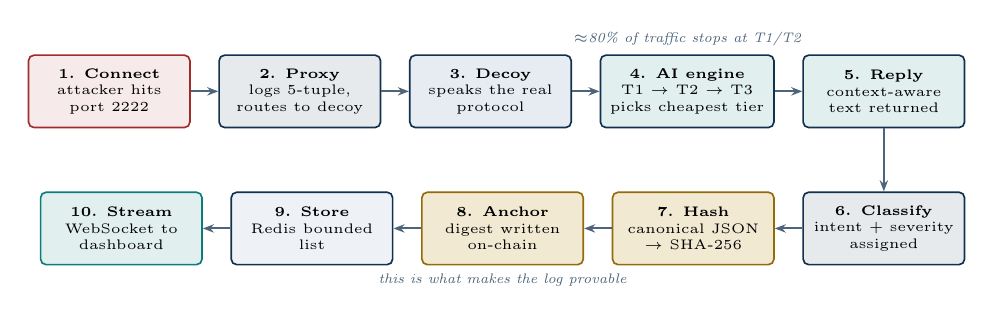
\begin{tikzpicture}[node distance=3.5mm]
    \tikzset{lifestep/.style={box, minimum width=2.05cm, minimum height=0.92cm, font=\tiny}}
    \node[lifestep, fill=crimson!10, draw=crimson] (s1) {\textbf{1. Connect}\\attacker hits\\port 2222};
    \node[lifestep, fill=navy!10, right=of s1]  (s2) {\textbf{2. Proxy}\\logs 5-tuple,\\routes to decoy};
    \node[lifestep, fill=steel!12, right=of s2] (s3) {\textbf{3. Decoy}\\speaks the real\\protocol};
    \node[lifestep, fill=teal!12, right=of s3]  (s4) {\textbf{4. AI engine}\\T1 $\rightarrow$ T2 $\rightarrow$ T3\\picks cheapest tier};
    \node[lifestep, fill=teal!12, right=of s4]  (s5) {\textbf{5. Reply}\\context-aware\\text returned};
    \node[lifestep, fill=navy!10, below=8mm of s5] (s6) {\textbf{6. Classify}\\intent + severity\\assigned};
    \node[lifestep, fill=amber!18, draw=amber!80!black, left=of s6] (s7) {\textbf{7. Hash}\\canonical JSON\\$\rightarrow$ SHA-256};
    \node[lifestep, fill=amber!18, draw=amber!80!black, left=of s7] (s8) {\textbf{8. Anchor}\\digest written\\on-chain};
    \node[lifestep, fill=mist, left=of s8] (s9) {\textbf{9. Store}\\Redis bounded\\list};
    \node[lifestep, fill=teal!12, draw=teal, left=of s9] (s10) {\textbf{10. Stream}\\WebSocket to\\dashboard};

    \draw[flow] (s1)--(s2); \draw[flow] (s2)--(s3); \draw[flow] (s3)--(s4); \draw[flow] (s4)--(s5);
    \draw[flow] (s5)--(s6);
    \draw[flow] (s6)--(s7); \draw[flow] (s7)--(s8); \draw[flow] (s8)--(s9); \draw[flow] (s9)--(s10);

    \node[lbl, above=0.5mm of s4] {$\approx$80\% of traffic stops at T1/T2};
    \node[lbl, below=0.5mm of s8] {this is what makes the log provable};
  \end{tikzpicture}
  \vspace{2pt}
  \takeaway{Steps 1--5 decide whether the attacker \emph{believes} us. Steps 6--10 decide whether we can \emph{prove} what they did. The two halves are independent, so they are evaluated independently.}
\end{frame}

% ============================== DECOYS ===============================
\begin{frame}{The Five Decoy Services}
  \vspace{-1pt}
  \centering\scriptsize
  \setlength{\tabcolsep}{4.5pt}\renewcommand{\arraystretch}{1.3}
  \begin{tabular}{@{}L{2.05cm} L{2.15cm} L{7.5cm}@{}}
    \hdrow \hc{Decoy} & \hc{Port / Protocol} & \hc{Role and bait}\\
    \altrow \textbf{shadow-shell} & 2222 / SSH & Real \texttt{asyncssh} server; accepts any credentials; shell prompt for \texttt{dbadmin@corp-prod-db-01}; every command routes through the AI engine\\
    \textbf{oracle-ai} & 8080 / REST & FastAPI \texttt{chat}/\texttt{predict} endpoints for a fictitious internal model --- prompt-injection bait\\
    \altrow \textbf{vault-sql} & 5433 / Postgres & Real seeded Postgres instance with synthetic records + honeytoken API keys (OpenAI / GitHub / AWS formats)\\
    \textbf{ledger-trap} & 8545 / JSON-RPC & Ethereum node decoy; static replies for common RPC calls, AI engine for uncommon ones\\
    \altrow \textbf{forge-ci} & 9090 / HTTP & Jenkins-style CI/CD endpoints faking a working pipeline --- supply-chain bait\\
    \bottomrule
  \end{tabular}
  \srcnote{Paper Section III.B}
  \takeaway{Each decoy is a \emph{real} server speaking a \emph{real} protocol --- the deception is in the content it returns, not in a fake socket. That is why generic protocol fingerprinting does not immediately expose it.}
\end{frame}

% ============================== 3-TIER ENGINE ========================
\begin{frame}{Three-Tier AI Response Engine}
  \framesubtitle{Expensive LLM calls are reserved for genuinely novel input.}
  \vspace{-2pt}
  \centering
  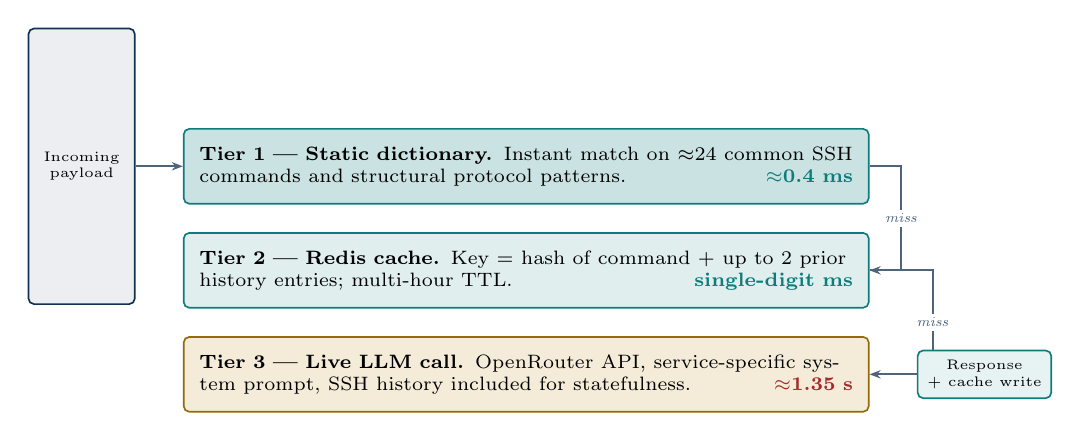
\begin{tikzpicture}
    \tikzset{tbox/.style={box, minimum width=8.7cm, minimum height=0.95cm, font=\scriptsize, align=left, text width=8.3cm}}
    \node[tbox, fill=teal!22, draw=teal] (a)
      {\textbf{Tier 1 --- Static dictionary.} Instant match on $\approx$24 common SSH commands and structural
       protocol patterns. \hfill \good{$\approx$0.4 ms}};
    \node[tbox, fill=teal!13, draw=teal, below=3.5mm of a] (b)
      {\textbf{Tier 2 --- Redis cache.} Key = hash of command + up to 2 prior history entries;
       multi-hour TTL. \hfill \good{single-digit ms}};
    \node[tbox, fill=amber!16, draw=amber!80!black, below=3.5mm of b] (c)
      {\textbf{Tier 3 --- Live LLM call.} OpenRouter API, service-specific system prompt, SSH history
       included for statefulness. \hfill \bad{$\approx$1.35 s}};

    \node[box, left=6mm of a, minimum height=3.5cm, minimum width=1.35cm, fill=navy!8, font=\tiny] (in)
      {Incoming\\payload};
    \draw[flow] (in.east) -- (a.west);
    \draw[flow] (a.east) -- ++(4mm,0) |- node[lbl, pos=0.25]{miss} (b.east);
    \draw[flow] (b.east) -- ++(8mm,0) |- node[lbl, pos=0.25]{miss} (c.east);
    \node[box, right=6mm of c, fill=teal!10, draw=teal, font=\tiny, minimum width=1.35cm] (out) {Response\\+ cache write};
  \end{tikzpicture}
  \vspace{2pt}

  \footnotesize
  \textbf{Intent classification:} keyword-based, 9 categories --- reconnaissance, privilege escalation,
  SQL injection, reverse shell, cryptomining, crypto theft, prompt injection, supply-chain, unknown.
  A deliberately simple rule-based baseline; Module 3 tests whether an LLM can beat it.
  \srcnote{Paper Section III.C--D}
\end{frame}

% ============================== BLOCKCHAIN ===========================
\begin{frame}{Blockchain-Anchored Logging}
  \framesubtitle{Removing the honeypot host from the trust boundary of its own forensic record.}
  \vspace{-3pt}
  \centering
  \begin{adjustbox}{max width=\textwidth, center}
  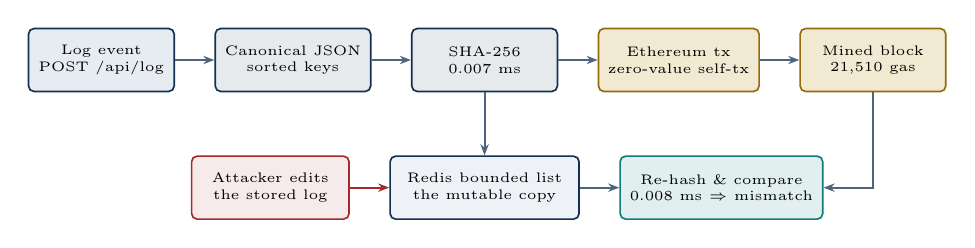
\begin{tikzpicture}[node distance=5mm]
    \tikzset{pbox/.style={box, minimum width=1.85cm, minimum height=0.8cm, font=\tiny}}
    \node[pbox, fill=steel!12] (e) {Log event\\\tiny{POST /api/log}};
    \node[pbox, fill=navy!10, right=of e] (c) {Canonical JSON\\\tiny{sorted keys}};
    \node[pbox, fill=navy!10, right=of c] (h) {SHA-256\\\tiny{0.007 ms}};
    \node[pbox, fill=amber!18, draw=amber!80!black, right=of h] (t) {Ethereum tx\\\tiny{zero-value self-tx}};
    \node[pbox, fill=amber!18, draw=amber!80!black, right=of t] (m) {Mined block\\\tiny{21{,}510 gas}};
    \draw[flow] (e)--(c); \draw[flow] (c)--(h); \draw[flow] (h)--(t); \draw[flow] (t)--(m);

    \node[pbox, fill=mist, below=8mm of h, minimum width=2.4cm] (s) {Redis bounded list\\\tiny{the mutable copy}};
    \node[pbox, fill=crimson!10, draw=crimson, left=of s, minimum width=2.0cm] (adv) {Attacker edits\\the stored log};
    \node[pbox, fill=teal!12, draw=teal, right=of s, minimum width=2.4cm] (v) {Re-hash \& compare\\\tiny{0.008 ms $\Rightarrow$ mismatch}};
    \draw[flow] (h.south) -- ++(0,-3mm) -| (s.north);
    \draw[flow, draw=crimson] (adv)--(s);
    \draw[flow] (s)--(v);
    \draw[flow] (m.south) |- (v.east);
  \end{tikzpicture}
  \end{adjustbox}
  \vspace{3pt}

  \begin{block}{\scriptsize Integrity test, run against the live stack}
    \scriptsize A log entry (digest \texttt{356b7496\ldots33a9a1}) was anchored, fetched back and re-hashed
    --- \good{identical}. A tampered copy (\texttt{"sudo cat /etc/shadow"} $\rightarrow$ \texttt{"ls -la"})
    produced digest \texttt{7530fb00\ldots0d9d394} --- \bad{mismatch}, so the edit is proven.
  \end{block}
  \srcnote{Paper Section III.E, V.D}
\end{frame}

% ============================== IMPLEMENTATION =======================
\begin{frame}{Implementation Stack --- What Actually Runs}
  \vspace{-2pt}
  \centering\scriptsize
  \setlength{\tabcolsep}{5pt}\renewcommand{\arraystretch}{1.16}
  \begin{tabular}{@{}L{2.4cm} L{4.15cm} L{5.05cm}@{}}
    \hdrow \hc{Layer} & \hc{Technology} & \hc{Notes}\\
    \altrow Edge proxy & Python \texttt{asyncio} TCP proxy & 5 public ports, per-connection logging\\
    Decoys & \texttt{asyncssh}, FastAPI, real PostgreSQL & 5 containers, real protocol servers\\
    \altrow AI engine & Static dict $\rightarrow$ Redis $\rightarrow$ OpenRouter & Llama-3.1-8B generator; pooled HTTP\\
    Backend & FastAPI + \texttt{web3.py} & classify, hash, anchor, broadcast\\
    \altrow Ledger & Ganache v7.9.2, chain ID 1337 & Ethereum-compatible, local\\
    Dashboard & React + WebSocket & live attack feed, intent timeline\\
    \altrow Orchestration & Docker Compose & one internal network, two exposed services\\
    Evaluation & Custom harnesses + LLM judge (70B) & judge model distinct from generator\\
    \bottomrule
  \end{tabular}
  \takeaway{Everything reported in this deck was measured against \emph{this running stack} --- real LLM calls, a real chain, a real database. No simulation, no hand-typed numbers.}
\end{frame}

% ============================== METHODOLOGY ==========================
\begin{frame}{Evaluation Methodology}
  \small
  Evaluated against the system's own \hl{static fast-path} (functionally equivalent to Cowrie)
  vs.\ its \hl{LLM-backed dynamic path}.
  \vspace{2pt}
  \begin{columns}[T,onlytextwidth]
    \begin{column}{0.49\textwidth}
      \footnotesize\textbf{\color{navy}Four metrics, kept separate}
      \begin{itemize}\setlength\itemsep{1.5pt}\footnotesize
        \item Latency / throughput (30 static, 20 dynamic trials)
        \item Response diversity --- fraction of distinct outputs per service
        \item LLM-judge realism --- independent 70B judge, 1--5 rubric, 30-payload sample
        \item Blockchain integrity --- direct tamper test
      \end{itemize}
    \end{column}
    \begin{column}{0.49\textwidth}
      \footnotesize\textbf{\color{navy}Four runs, each scaling realism}
      \begin{enumerate}\setlength\itemsep{1.5pt}\footnotesize
        \item 100 hand-written payloads (baseline)
        \item Same dataset, after an optimisation pass
        \item 200 real, publicly-documented payloads
        \item 1{,}328 real payloads (scaled corpora)
      \end{enumerate}
    \end{column}
  \end{columns}
  \vspace{3pt}
  \takeaway{Explicitly \emph{not} a single composite accuracy figure. Trade-offs and failures are reported, not hidden --- which is exactly how the two most interesting results in this deck were found.}
  \srcnote{Paper Section IV}
\end{frame}

% ============================== RUN 1 ================================
\begin{frame}{Module 1, Run 1 --- Initial Baseline (100 Hand-Written Payloads)}
  \vspace{-1pt}
  \centering\small
  \setlength{\tabcolsep}{9pt}\renewcommand{\arraystretch}{1.3}
  \begin{tabular}{@{}l r r@{}}
    \hdrow \hc{Metric} & \hc{Static path} & \hc{Dynamic (LLM) path}\\
    \altrow Mean latency & 0.4 ms & 4{,}028 ms (4.03 s)\\
    Median latency & 0.4 ms & 3{,}529 ms (3.53 s)\\
    \altrow Throughput (req/s) & 2{,}500 & 0.25\\
    Diversity ratio (mean) & $\approx$0 & 0.99 (0.95--1.00)\\
    \bottomrule
  \end{tabular}
  \vspace{5pt}

  \footnotesize LLM-judge realism: \hl{4.38 / 5} ($\sigma = 1.28$, $n = 24$ of 30 parsed)
  \srcnote{Table II, paper Section V.A}
  \takeaway{The trade-off is stark and it is the whole story of this project: the LLM path is $\approx$10{,}000$\times$ slower, and $\approx$10{,}000$\times$ more varied. Everything that follows is about narrowing the first gap without losing the second.}
\end{frame}

% ============================== RUN 2 ================================
\begin{frame}{Module 1, Run 2 --- Optimisation Pass}
  \footnotesize
  Three fixes identified by profiling:
  \begin{itemize}\setlength\itemsep{1pt}
    \item \textbf{HTTP connection pooling} --- we were opening a fresh TCP+TLS handshake to OpenRouter on every request.
    \item \textbf{Generation-length cap} tuned 150 $\rightarrow$ 60 tokens (150 tok $\approx$5.3 s, 80 tok $\approx$3.4 s, 40 tok $\approx$2.0 s --- generation length dominates latency).
    \item \textbf{Static SSH dictionary widened} with 12 more reconnaissance commands.
  \end{itemize}
  \par\vspace{2pt}
  \centering\scriptsize
  \setlength{\tabcolsep}{8pt}\renewcommand{\arraystretch}{1.22}
  \begin{tabular}{@{}l r r c@{}}
    \hdrow \hc{Metric} & \hc{Before} & \hc{After} & \hc{Change}\\
    \altrow Dynamic mean latency & 4.03 s & 1.35 s & \good{$\approx$3$\times$ faster}\\
    Dynamic throughput (seq.) & 0.25 rps & 0.74 rps & \good{$\approx$3$\times$}\\
    \altrow Static throughput & 2{,}500 rps & 3{,}333 rps & \good{+33\%}\\
    LLM-judge realism & 4.38/5 (24/30) & 4.00/5 (30/30) & \bad{$-$0.38}\\
    \bottomrule
  \end{tabular}
  \srcnote{Table III, paper Section V.B}
  \takeaway{Speed was bought with realism --- shorter generations are less convincing. We report the loss rather than quoting only the 3$\times$ speed-up.}
\end{frame}

% ============================== LATENCY CHART ========================
\begin{frame}{Latency Comparison --- Before vs.\ After}
  \vspace{-2pt}
  \centering
  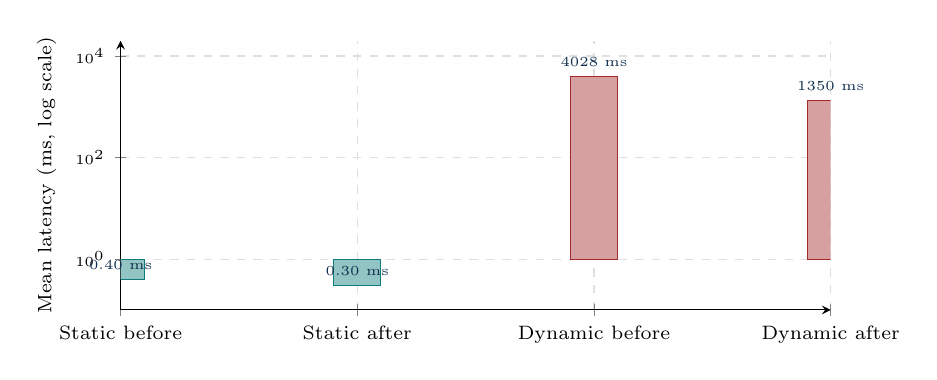
\begin{tikzpicture}
    \begin{axis}[
      width=10.6cm, height=5.0cm,
      ybar, bar width=17pt,
      ymode=log, log basis y={10},
      ymin=0.1, ymax=20000,
      ylabel={\scriptsize Mean latency (ms, log scale)},
      symbolic x coords={Static before, Static after, Dynamic before, Dynamic after},
      xtick={Static before, Static after, Dynamic before, Dynamic after},
      xticklabel style={font=\scriptsize},
      yticklabel style={font=\tiny},
      ylabel style={font=\scriptsize},
      nodes near coords, nodes near coords style={font=\tiny, color=navy},
      point meta=explicit symbolic,
      grid=major, grid style={dashed, gray!25},
      axis lines=left,
      ]
      \addplot[fill=teal!45, draw=teal, bar shift=0pt] coordinates {
        (Static before,0.4)[0.40 ms] (Static after,0.3)[0.30 ms]};
      \addplot[fill=crimson!45, draw=crimson, bar shift=0pt] coordinates {
        (Dynamic before,4028)[4028 ms] (Dynamic after,1350)[1350 ms]};
    \end{axis}
  \end{tikzpicture}
  \srcnote{Fig.\ 1, paper Section V.B}
  \takeaway{Four orders of magnitude separate the two paths. This is why the tiering matters: routing 80\% of traffic to the left-hand bars is what makes the system usable at all.}
\end{frame}

% ============================== POOLING ==============================
\begin{frame}{Decoy-Layer Connection Pooling --- All Five Decoys}
  \vspace{-1pt}
  \centering\small
  \setlength{\tabcolsep}{10pt}\renewcommand{\arraystretch}{1.3}
  \begin{tabular}{@{}l r r r@{}}
    \hdrow \hc{Decoy} & \hc{Before (mean)} & \hc{After (mean)} & \hc{$\Delta$}\\
    \altrow oracle-ai & 6.15 ms & 4.28 ms & \good{$-$30.4\%}\\
    vault-sql & 0.69 ms & 0.41 ms & \good{$-$41.4\%}\\
    \altrow ledger-trap & 5.96 ms & 4.20 ms & \good{$-$29.5\%}\\
    forge-ci & 6.95 ms & 6.71 ms & $-$3.4\%\\
    \altrow shadow-shell & 7.91 ms & 4.64 ms & \good{$-$41.3\%}\\
    \bottomrule
  \end{tabular}
  \srcnote{Table IV, paper Section V.C}
  \takeaway{Real and consistent improvement on 4 of 5 decoys. \texttt{forge-ci} barely moves --- and that is the correct result, because it always routes through the AI engine regardless of decoy-layer pooling.}
\end{frame}

% ============================== RUNS 3-4 =============================
\begin{frame}{Module 1, Runs 3--4 --- Real-World Payload Datasets}
  \footnotesize
  The hand-written dataset was replaced with \hl{real, publicly-documented attack payloads}
  (payload-box, PayloadsAllTheThings, SecLists), scaled 100 $\rightarrow$ 200 $\rightarrow$ 1{,}328.
  \par\vspace{3pt}
  \centering\scriptsize
  \setlength{\tabcolsep}{12pt}\renewcommand{\arraystretch}{1.24}
  \begin{tabular}{@{}l r r@{}}
    \hdrow \hc{Metric} & \hc{200-item set} & \hc{1{,}328-item set}\\
    \altrow Dynamic latency (mean) & 2.06 s & 1.95 s\\
    Concurrent throughput (10 sessions) & 1.62 req/s & 3.05 req/s\\
    \altrow Response diversity --- ssh & 0.925 & 0.964\\
    Response diversity --- sql & 1.00 & 0.978\\
    \altrow Response diversity --- web3 & 0.80 & 0.833\\
    Response diversity --- cicd & 0.90 & 1.00\\
    \altrow Response diversity --- api & 0.70 & \bad{0.46}\\
    LLM-judge realism (mean) & 4.03 / 5 & \bad{3.37 / 5}\\
    \bottomrule
  \end{tabular}
  \srcnote{Table VI, paper Section V.E--F}
  \takeaway{Latency and throughput \emph{improved} at scale; realism \emph{degraded}. The degradation is not spread evenly --- it is concentrated in one service, which is the subject of the next three slides.}
\end{frame}

% ============================== DIVERSITY CHART ======================
\begin{frame}{Response Diversity by Decoy Service}
  \vspace{-2pt}
  \centering
  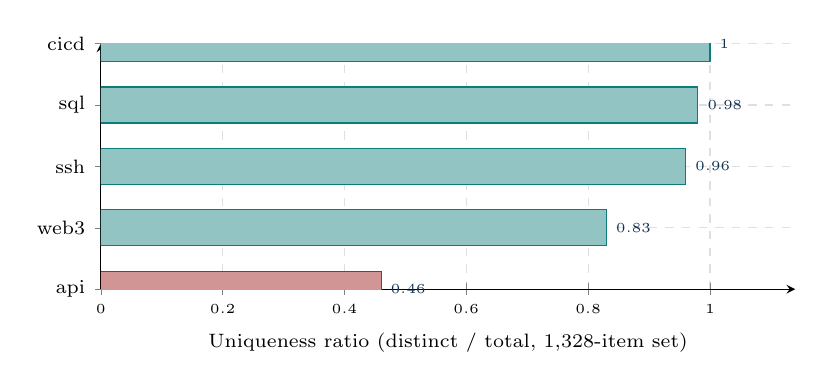
\begin{tikzpicture}
    \begin{axis}[
      width=10.4cm, height=4.7cm,
      xbar, bar width=13pt,
      xmin=0, xmax=1.14,
      symbolic y coords={api, web3, ssh, sql, cicd},
      ytick={api, web3, ssh, sql, cicd}, yticklabel style={font=\scriptsize},
      xticklabel style={font=\tiny},
      xlabel={\scriptsize Uniqueness ratio (distinct / total, 1{,}328-item set)},
      xlabel style={font=\scriptsize},
      nodes near coords, nodes near coords style={font=\tiny, color=navy},
      grid=major, grid style={dashed, gray!25}, axis lines=left,
      ]
      \addplot[fill=crimson!50, draw=crimson, bar shift=0pt] coordinates {(0.46,api)};
      \addplot[fill=teal!45, draw=teal, bar shift=0pt] coordinates {(0.83,web3) (0.96,ssh) (0.98,sql) (1.00,cicd)};
    \end{axis}
  \end{tikzpicture}
  \vspace{-2pt}

  \footnotesize
  \texttt{api} is the clear outlier --- on real XXE / Log4Shell strings the model collapses to a generic
  \emph{``invalid request''} reply instead of emulating a plausible vulnerable-parser response.
  \srcnote{Fig.\ 5, paper Section V.C, V.F}
\end{frame}

% ============================== BUG ==================================
\begin{frame}{The Benchmark-Harness Bug}
  \framesubtitle{A genuine measurement bug, found and fixed during the real-dataset re-run.}
  \footnotesize
  \begin{itemize}\setlength\itemsep{2pt}
    \item The concurrent-throughput benchmark \textbf{reused payloads already sent once earlier in the same run}.
    \item Because the Redis cache key derives from \emph{command + history}, these were guaranteed cache hits ---
      so the ``800 req/s'' figure measured \textbf{Redis latency, not LLM latency}.
    \item \textbf{Fix:} append a fresh UUID nonce to every payload immediately before firing the concurrent batch.
  \end{itemize}
  \par\vspace{4pt}
  \centering\small
  \setlength{\tabcolsep}{12pt}\renewcommand{\arraystretch}{1.3}
  \begin{tabular}{@{}l r r@{}}
    \hdrow \hc{Metric} & \hc{First reported (buggy)} & \hc{Corrected}\\
    \altrow Concurrent throughput (10 sessions) & 800.3 req/s & 3.05 req/s\\
    Mean per-request latency & 8.2 ms & 2.62 s\\
    \bottomrule
  \end{tabular}
  \srcnote{Table V, paper Section V.E}
  \takeaway{Reported explicitly rather than silently substituted. A three-order-of-magnitude measurement error is itself a methodological finding --- and a warning for anyone benchmarking a cached LLM pipeline.}
\end{frame}

% ============================== REALISM DIST =========================
\begin{frame}{Realism Score Distribution (Post-Optimisation, $n=30$)}
  \vspace{-2pt}
  \centering
  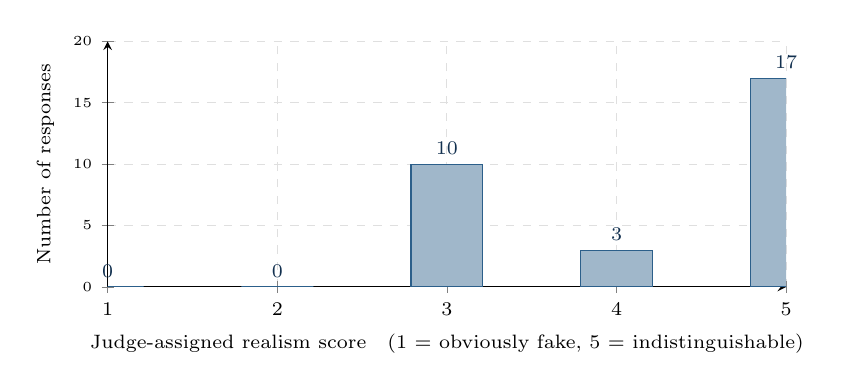
\begin{tikzpicture}
    \begin{axis}[
      width=10.2cm, height=4.7cm,
      ybar, bar width=26pt,
      ymin=0, ymax=20,
      xlabel={\scriptsize Judge-assigned realism score \; (1 = obviously fake, 5 = indistinguishable)},
      ylabel={\scriptsize Number of responses},
      xlabel style={font=\scriptsize}, ylabel style={font=\scriptsize},
      symbolic x coords={1,2,3,4,5}, xtick=data,
      xticklabel style={font=\scriptsize}, yticklabel style={font=\tiny},
      nodes near coords, nodes near coords style={font=\scriptsize, color=navy},
      grid=major, grid style={dashed, gray!25}, axis lines=left,
      ]
      \addplot[fill=steel!45, draw=steel] coordinates {(1,0) (2,0) (3,10) (4,3) (5,17)};
    \end{axis}
  \end{tikzpicture}
  \vspace{-2pt}

  \footnotesize
  Bimodal, not centred: \good{17 responses are judged indistinguishable from a real system},
  while 10 sit at a mediocre 3/5. \textbf{Zero} responses scored 1 or 2 at this dataset scale ---
  a property that does \emph{not} survive to the 1{,}328-item set.
  \srcnote{Fig.\ 3, paper Section V.B}
\end{frame}

% ============================== API FAILURE ==========================
\begin{frame}{Key Finding --- The API Decoy's Realism Failure}
  \footnotesize
  At the 1{,}328-item scale, \bad{9 of 11} sampled \texttt{api} responses scored 1--2 / 5 ---
  versus near-uniform 5/5 for \texttt{ssh}, \texttt{sql} and \texttt{web3} in the same sample.
  \vspace{3pt}
  \begin{alertblock}{\scriptsize Most consequential result}
    \scriptsize One sampled response was found to contain an \textbf{explicit AI safety disclaimer}
    (``Contains an explicit disclaimer about not generating harmful responses'') --- a
    \emph{hard deception failure}, not a minor realism deduction. It signals ``this is not a real
    system'' to exactly the attentive attacker the framework is designed to hold.
  \end{alertblock}
  \vspace{1pt}
  \begin{itemize}\setlength\itemsep{1.5pt}
    \item This failure was \textbf{invisible} in the 100-payload and even the 200-payload runs ---
      it only became unambiguous at the largest scale. \emph{Small benchmarks hide structural faults.}
    \item \textbf{Root cause:} the hosted model's own safety training bleeds through the deception
      persona on XML / JNDI-shaped adversarial input.
    \item \textbf{Actionable fix (specified, not yet applied):} XXE / Log4Shell / SSRF-aware few-shot
      examples plus an explicit anti-disclaimer instruction in \texttt{oracle-ai}'s system prompt.
  \end{itemize}
  \srcnote{Paper Section V.F, VI}
\end{frame}

% ============================== MODULE 2 =============================
\begin{frame}{Module 2 --- Tamper-Evident Audit Trail, Measured}
  \framesubtitle{300 anchored events, 500 tampering trials, against a live Ganache chain --- not a simulation.}
  \vspace{-2pt}
  \centering\scriptsize
  \setlength{\tabcolsep}{7pt}\renewcommand{\arraystretch}{1.16}
  \begin{tabular}{@{}L{4.55cm} R{2.95cm} L{4.55cm}@{}}
    \hdrow \hc{Measurement} & \hc{Result} & \hc{Reading}\\
    \altrow Anchor latency (mean / p95) & 10.86 / 14.42 ms & on-chain commit dominates\\
    SHA-256 hashing alone & 0.007 ms & cryptography is \emph{free} here\\
    \altrow Verification (re-hash) & 0.008 ms & checking is instant\\
    Gas per anchor & 21{,}510 & a minimal-payload Ethereum tx\\
    \altrow Anchoring success rate & 300 / 300 = 100\% & no dropped evidence\\
    Tamper detection (500 trials) & \good{500 detected, 0 FP} & 100\% detection rate\\
    \altrow Throughput seq. / conc.\ (10) & 92.1 / 141.2 per s & concurrency gives 1.53$\times$\\
    On-chain retrievability & digest recovered & anyone can verify independently\\
    \bottomrule
  \end{tabular}
  \srcnote{Paper 3 (Ganache v7.9.2, chain ID 1337); measured 2026-08-18}
  \takeaway{Forensic integrity costs $\approx$11 ms per event and detects 100\% of edits. Compared with a 1{,}350 ms LLM response, tamper-evidence is effectively free.}
\end{frame}

% ============================== MODULE 3 =============================
\begin{frame}{Module 3 --- Can an LLM Replace the Rule-Based Classifier?}
  \framesubtitle{121 hand-labelled payloads, 9 intent categories, head-to-head on identical input.}
  \vspace{-3pt}
  \centering
  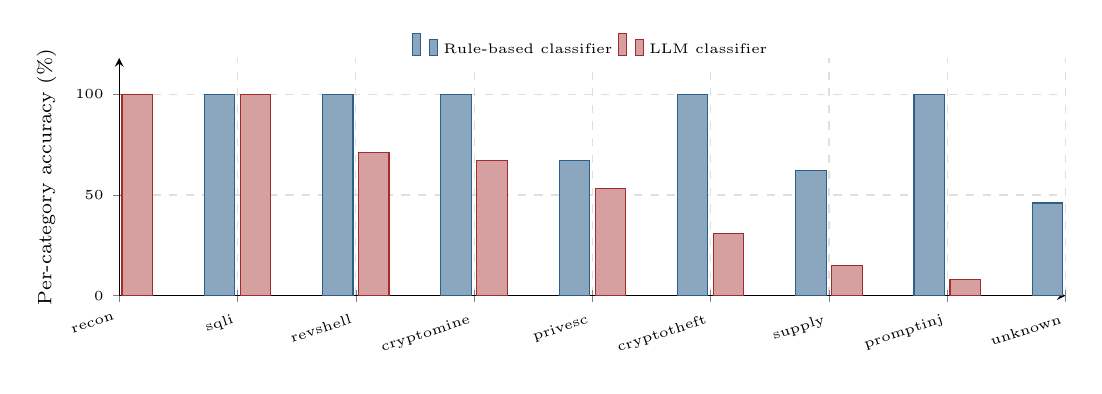
\begin{tikzpicture}
    \begin{axis}[
      width=13.6cm, height=4.6cm,
      ybar, bar width=11pt,
      ymin=0, ymax=118,
      ylabel={\scriptsize Per-category accuracy (\%)},
      ylabel style={font=\scriptsize},
      symbolic x coords={recon, sqli, revshell, cryptomine, privesc, cryptotheft, supply, promptinj, unknown},
      xtick=data, xticklabel style={font=\tiny, rotate=18, anchor=north east},
      yticklabel style={font=\tiny},
      legend style={font=\tiny, at={(0.5,1.13)}, anchor=north, legend columns=2, draw=none},
      grid=major, grid style={dashed, gray!25}, axis lines=left,
      ]
      \addplot[fill=steel!55, draw=steel] coordinates
        {(recon,93) (sqli,100) (revshell,100) (cryptomine,100) (privesc,67) (cryptotheft,100) (supply,62) (promptinj,100) (unknown,46)};
      \addplot[fill=crimson!45, draw=crimson] coordinates
        {(recon,100) (sqli,100) (revshell,71) (cryptomine,67) (privesc,53) (cryptotheft,31) (supply,15) (promptinj,8) (unknown,0)};
      \legend{Rule-based classifier, LLM classifier}
    \end{axis}
  \end{tikzpicture}
  \vspace{-1pt}

  \scriptsize
  Overall: rule-based \good{85.1\%} vs.\ LLM \bad{50.4\%}; the two agree on only 56.2\% of payloads.
  The LLM's default fallback label is ``reconnaissance'' --- it mislabelled \bad{all 13} benign/unknown
  payloads as active threats. Every verdict was anchored (121/121); 40/40 tamper trials detected.
  \srcnote{Paper 4; Llama-3.1-8B, 1{,}669 ms mean LLM call + 24.8 ms anchor}
\end{frame}

\begin{frame}{Module 3 --- Why This Negative Result Matters}
  \footnotesize
  \begin{itemize}\setlength\itemsep{4pt}
    \item The obvious design instinct --- ``replace the brittle keyword rules with an LLM'' --- is
      \textbf{measurably wrong here}, by 35 percentage points, on the same inputs.
    \item The errors are \textbf{not evenly distributed}. They cluster in exactly the categories where a
      wrong answer is most expensive: prompt injection (8\%), supply-chain (15\%), crypto theft (31\%),
      and benign traffic (0\%).
    \item Over-classifying benign traffic as an active threat produces \textbf{alert fatigue}, which
      erodes operator trust more quietly than a missed detection does.
    \item This is why we anchor the \emph{verdict}, not just the raw event: an AI artifact this fallible
      will sometimes be wrong, and \textbf{a wrong verdict that can be quietly edited afterwards is worse
      than no verdict at all} --- it launders an error into something that looks authoritative.
  \end{itemize}
  \takeaway{Design principle we can defend with data: \emph{an AI classifier in a security-decision role should be treated as a fallible witness, not as ground truth.}}
\end{frame}

% ============================== MODULE 4 =============================
\begin{frame}{Module 4 --- Federated Threat Intelligence Without a Hub}
  \framesubtitle{Five concurrent honeypot nodes, 60 IOCs each, 300 anchored events on a live chain.}
  \footnotesize
  \textbf{Idea:} a campaign touches many decoys, but each honeypot sees only a fragment. The usual
  fix is a central threat-intel server --- the one machine an adversary must reach to blind the whole
  network. \hl{We remove it}: each node hashes its own indicators, tags the digest with its identity,
  and writes to a shared chain. No node ever calls another.
  \par\vspace{2pt}
  \centering\tiny
  \setlength{\tabcolsep}{7pt}\renewcommand{\arraystretch}{1.20}
  \begin{tabular}{@{}L{4.75cm} R{2.85cm} L{4.45cm}@{}}
    \hdrow \hc{Measurement} & \hc{Result} & \hc{Reading}\\
    \altrow Anchor latency (mean / p95) & 8.44 / 11.06 ms & per-node band 7.93--9.19 ms\\
    Propagation to a blind observer & 1.94 ms, 40/40 & correlation without coordination\\
    \altrow Cold-start reconstruction & all 220 IOCs & from chain history alone\\
    Corroboration accuracy & 195 single / 25 shared & no false merges or misses\\
    \altrow Compromised-node forgery & \good{forgery caught} & original digest still on-chain\\
    Throughput --- 5 nodes vs.\ 1 & 228.6 vs.\ 98.6 per s & \good{2.32$\times$} from concurrency\\
    \bottomrule
  \end{tabular}
  \srcnote{Paper 5; 35\% ground-truth overlap from a 25-IOC campaign pool}
  \takeaway{A fresh node that never contacted any peer rebuilds the full campaign picture by reading the ledger --- the single point of failure is genuinely gone, not merely replicated.}
\end{frame}

% ============================== STATUS ===============================
\begin{frame}{Project Status --- Approximately 70\% Complete}
  \vspace{-3pt}
  \centering
  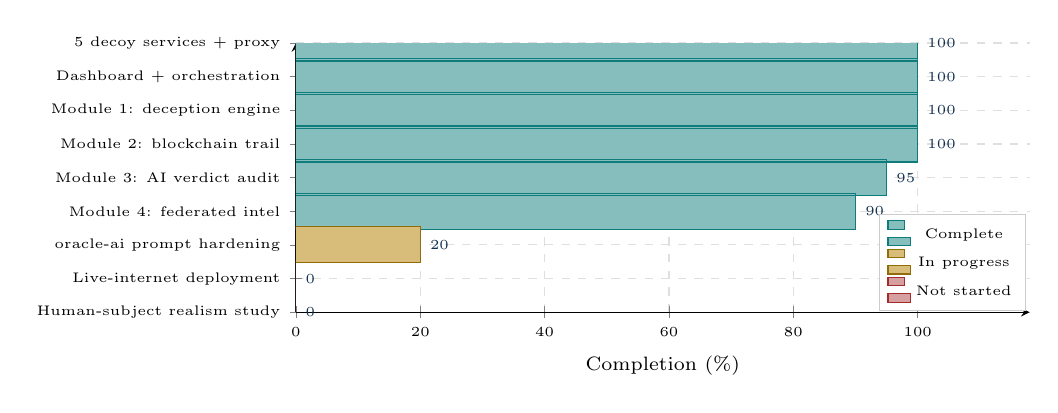
\begin{tikzpicture}
    \begin{axis}[
      width=10.9cm, height=5.0cm,
      xbar, bar width=13pt, bar shift=0pt,
      xmin=0, xmax=118,
      symbolic y coords={
        {Human-subject realism study}, {Live-internet deployment},
        {oracle-ai prompt hardening}, {Module 4: federated intel},
        {Module 3: AI verdict audit}, {Module 2: blockchain trail},
        {Module 1: deception engine}, {Dashboard + orchestration},
        {5 decoy services + proxy}},
      ytick={{Human-subject realism study},{Live-internet deployment},
             {oracle-ai prompt hardening},{Module 4: federated intel},
             {Module 3: AI verdict audit},{Module 2: blockchain trail},
             {Module 1: deception engine},{Dashboard + orchestration},
             {5 decoy services + proxy}},
      yticklabel style={font=\tiny},
      xticklabel style={font=\tiny},
      xlabel={\scriptsize Completion (\%)}, xlabel style={font=\scriptsize},
      nodes near coords, nodes near coords style={font=\tiny, color=navy},
      legend style={font=\tiny, at={(0.995,0.005)}, anchor=south east, draw=gray!40, fill=white},
      grid=major, grid style={dashed, gray!25}, axis lines=left,
      ]
      \addplot[fill=teal!50, draw=teal, bar shift=0pt] coordinates {
        (100,{5 decoy services + proxy}) (100,{Dashboard + orchestration})
        (100,{Module 1: deception engine}) (100,{Module 2: blockchain trail})
        (95,{Module 3: AI verdict audit}) (90,{Module 4: federated intel})};
      \addplot[fill=amber!55, draw=amber!80!black, bar shift=0pt] coordinates {(20,{oracle-ai prompt hardening})};
      \addplot[fill=crimson!45, draw=crimson, bar shift=0pt] coordinates {
        (0,{Live-internet deployment}) (0,{Human-subject realism study})};
      \legend{Complete, In progress, Not started}
    \end{axis}
  \end{tikzpicture}
  \vspace{-3pt}

  \scriptsize
  \good{Done:} full running stack, four measured evaluation modules, four paper drafts, all
  benchmarks reproducible against the live system. \quad
  \bad{Remaining:} prompt hardening + re-measurement, human-subject validation, longitudinal
  live deployment, learned intent classifier.
\end{frame}

% ============================== DISCUSSION ===========================
\begin{frame}{Discussion --- What the Numbers Actually Mean}
  \footnotesize
  \begin{itemize}\setlength\itemsep{3.5pt}
    \item \textbf{Not a drop-in replacement} for high-volume, low-interaction scanning honeypots ---
      static-path systems remain appropriate there, and we say so.
    \item \textbf{Targeted use case:} high-interaction deception against a human operator or a
      sophisticated, low-volume tool, where multi-second latency is plausibly attributable to
      network or server load.
    \item \textbf{Concurrency is real but modest:} 10 concurrent sessions complete in 3.28 s
      wall-clock (not $\approx$19.5 s) --- but far short of the originally (buggy) reported capacity.
    \item \textbf{The AI-persona failure is structural, not incidental:} any decoy built on a hosted,
      safety-tuned model inherits an alignment layer that is \emph{directly adversarial} to the
      deception goal on concerning inputs.
    \item \textbf{Blockchain anchoring assumes the ledger is outside attacker reach} --- reasonable for
      an internal Ganache deployment; not evaluated against an adversary who also compromises the
      chain client.
    \item \textbf{The cheap component won.} Across two independent experiments, the simple deterministic
      layer (static dictionary; keyword classifier) outperformed the sophisticated one on its own terms.
  \end{itemize}
  \srcnote{Paper Section VI}
\end{frame}

% ============================== LIMITATIONS ==========================
\begin{frame}{Limitations \& Future Work}
  \scriptsize
  \textbf{\color{navy}Limitations we acknowledge}
  \begin{itemize}\setlength\itemsep{1.5pt}
    \item LLM-judge realism is an \emph{automated proxy} --- needs human-subject validation
      (protocol specified in paper Appendix A, not yet executed).
    \item Real-payload datasets (up to 1{,}328 items) are still \emph{not live-traffic captures} ---
      no multi-step sessions, timing, or evasion behaviour.
    \item \texttt{web3} and \texttt{cicd} datasets remain small (18 and 10 payloads) --- no comparably
      large real corpus exists for those surfaces; a genuine coverage gap.
    \item Intent classification is keyword-based --- will misclassify obfuscated or novel patterns.
    \item Federated results come from a \emph{single local chain} with simulated nodes --- not a
      geographically distributed deployment with real consensus latency and partitions.
    \item No longitudinal live-internet deployment; concurrency tested only at a single burst level.
  \end{itemize}
  \vspace{2pt}
  \textbf{\color{navy}Next steps, in priority order}
  \begin{enumerate}\setlength\itemsep{1.5pt}
    \item Rewrite \texttt{oracle-ai}'s system prompt with XXE/JNDI-aware few-shot examples and an
      explicit anti-disclaimer instruction, then \emph{re-measure} the realism score.
    \item Replace the keyword classifier with a learned classifier and re-run the Module 3 head-to-head.
    \item Execute the human-subject realism protocol; then a supervised live deployment.
  \end{enumerate}
\end{frame}

% ============================== CONCLUSION ===========================
\begin{frame}{Conclusion}
  \footnotesize
  \begin{enumerate}\setlength\itemsep{3pt}
    \item We built and ran a \hl{five-protocol, LLM-driven deception framework} behind one shared
      three-tier response engine --- the first to apply a single LLM engine uniformly across
      heterogeneous protocols.
    \item We made its forensic record \hl{provable independently of the honeypot host}:
      100\% tamper detection over 500 trials at $\approx$11 ms per anchored event.
    \item We extended that discipline to the \hl{AI's own verdicts}, and then showed --- with data ---
      that those verdicts are wrong half the time, which is precisely why they must be anchored.
    \item We removed the \hl{central threat-intelligence hub}, showing that five independent nodes can
      corroborate a campaign by reading a shared ledger, with no node ever calling another.
    \item Throughout, we \hl{reported the failures}: a 3-order-of-magnitude benchmark bug, a realism
      regression bought with speed, and a hard deception failure caused by the model's own safety
      training.
  \end{enumerate}
  \takeaway{The honest negative results are the contribution the field is missing --- and they only became visible because we scaled the evaluation instead of stopping at a favourable number.}
\end{frame}

% ============================== REFERENCES ===========================
\begin{frame}{References I}
  \scriptsize
  \begin{enumerate}\setlength\itemsep{2.5pt}
    \item A. Vetterl and R. Clayton, ``Bitter Harvest: Systematically Fingerprinting Low- and
      Medium-interaction Honeypots at Internet Scale,'' \emph{Proc. 12th USENIX WOOT}, 2018.
    \item ``Gotta Catch 'em All: A Multistage Framework for Honeypot Fingerprinting,''
      \emph{ACM Digital Threats: Research and Practice}, 2023, arXiv:2109.10652.
    \item M. Slad\'{i}\'{c}, V. Valeros, C. Catania and S. Garcia, ``LLM in the Shell: Generative
      Honeypots,'' \emph{Proc. IEEE EuroS\&PW}, 2024, arXiv:2309.00155.
    \item Z. Wang et al., ``HoneyGPT: Breaking the Trilemma in Terminal Honeypots with Large
      Language Model,'' arXiv:2406.01882, 2024.
    \item F. McKee and D. Noever, ``Chatbots in a Honeypot World,'' arXiv:2301.03771, 2023.
    \item ``LLM Honeypot: Leveraging Large Language Models as Advanced Interactive Honeypot
      Systems,'' arXiv:2409.08234, 2024.
    \item ``Blockchain-Based Evidence Tracking System for Forensic Integrity and Secure Chain of
      Custody,'' IEEE, 2025.
    \item ``Blockchain-based tamper-proof and transparent investigation model for cloud VMs,''
      \emph{The Journal of Supercomputing}, Springer, 2022.
  \end{enumerate}
\end{frame}

\begin{frame}{References II}
  \scriptsize
  \begin{enumerate}\setlength\itemsep{2.5pt}\setcounter{enumi}{8}
    \item ``A novel intelligent cyber threat detection system with blockchain-enforced immutable
      forensic auditability,'' \emph{PeerJ Computer Science}, 2025.
    \item MITRE, ``MITRE Engage: A Framework and Community for Cyber Deception,'' 2022.
    \item Cowrie SSH/Telnet Honeypot, GitHub repository.
    \item ``SoK: Honeypots and Large Language Models --- Systematization of a Growing
      Intersection,'' arXiv:2510.25939, 2025.
    \item MISP --- Open Source Threat Intelligence Platform and Open Standards for Threat
      Information Sharing.
    \item OASIS, ``STIX / TAXII: Structured Threat Information Expression and Trusted Automated
      Exchange of Intelligence Information,'' Version 2.1, 2021.
  \end{enumerate}
\end{frame}

% ============================== THANK YOU ============================
{\setbeamertemplate{footline}{}
\begin{frame}[plain]
  \vfill
  \begin{center}
    {\color{navy}\rule{0.6\textwidth}{1pt}}\\[10pt]
    {\Large\color{navy}\bfseries Thank You}\\[8pt]
    {\small\color{steel} Questions and discussion}\\[10pt]
    {\color{navy}\rule{0.6\textwidth}{1pt}}\\[14pt]
    {\scriptsize\color{grayline} Team 58 \quad$\cdot$\quad Guide: Dr.\ Radhika G}
  \end{center}
  \vfill
\end{frame}}

\end{document}
